\documentclass[aspectratio=169,10pt]{beamer}
\usepackage[T1]{fontenc}
\usepackage{lmodern,graphicx,booktabs,tabularx,xcolor}
\definecolor{ink}{HTML}{20303C}
\definecolor{green}{HTML}{16836B}
\setbeamercolor{normal text}{fg=ink,bg=white}
\setbeamercolor{structure}{fg=green}
\setbeamertemplate{navigation symbols}{}
\setbeamertemplate{footline}[frame number]
\setbeamersize{text margin left=8mm,text margin right=8mm}
\renewcommand{\arraystretch}{1.15}
\newcommand{\oldasset}[1]{assets/transport_ft_with_hole/#1}
\newcommand{\asset}[1]{assets/acceptance_study/#1}
\newcommand{\ToyTracks}{2,624}
\newcommand{\FieldIntegral}{-4.1856}

\newcommand{\InventoryRows}{
TV & 100 & 50 & -288.0--558.1 \\
RICH1 & 2 & 2 & 795.0--2237.2 \\
UP & 16 & 4 & 2314.0--2656.0 \\
MP & 5 & 5 & 7665.5--9132.5 \\
FT & 12 & 12 & 7902.7--9384.7 \\
RICH2 & 2 & 2 & 9487.5--11839.2 \\
PicoCal & 2 & 2 & 12565.9--12601.0 \\
MUON & 4 & 4 & 15270.0--18870.0 \\
}

\title{LHCb Geometry Acceptance Studies}
\subtitle{FT\_withHole, MP, three UP variants and TV emulation}
\date{19 October 2026}
\begin{document}

\begin{frame}
\titlepage
\centering Six detector setups, each evaluated for MagUp and MagDown
\end{frame}

\begin{frame}{Main comparison: six geometries, two polarities}
\centering
\begin{tabular}{lcc}
\toprule UP variant & FT T1/T2/T3 & FT acceptance \\
\midrule
GDML nominal & 8/8/10 or 10/10/12 & FT\_withHole \\
Y8: top/bottom cutoff & 8/8/10 or 10/10/12 & FT\_withHole \\
Y8X6: additional left/right cutoff & 8/8/10 or 10/10/12 & FT\_withHole \\
\bottomrule
\end{tabular}\par
\vspace{5mm}
\begin{itemize}
\item Compare track-by-track \texttt{nFT}, \texttt{nMP}, and their combined \texttt{hasMT} cut.
\item Compare \texttt{nUP} across the three UP border variants.
\item Store TV cuts separately: \texttt{hasTV\_3Hits}, \texttt{hasTV\_4Hits}.
\item Every column carries a geometry suffix and, when both are run, a polarity suffix.
\end{itemize}
\end{frame}

\begin{frame}{Physical surfaces and counting layers}
\centering
\begin{tabular}{lrrr}
\toprule Detector & Surfaces & Logical layers & Global $z$ [mm] \\
\midrule
\InventoryRows
\bottomrule
\end{tabular}\par
\vspace{3mm}
\small A logical layer fires if any of its surfaces contains the track at that
surface's own $z$. Upstream surfaces do not fire. Multiple sensors in one
module do not create multiple counted layers.
\end{frame}

\begin{frame}{UP variants: same 16 surfaces and four counting layers}
\centering
\includegraphics[width=\textwidth,height=.68\textheight,keepaspectratio]{\oldasset{up_variants.pdf}}\par
\small Actual stored XY masks, not ideal box replacements. Crops preserve the
sensor pattern and beam exclusion; dimensions and central holes are quoted above.\\[2mm]
The four logical layer centres are 2317.5, 2372.5, 2597.5 and 2652.5 mm.
Each contains four nearby source surfaces.
\end{frame}

\begin{frame}{FT\_withHole subtracts the joined MP acceptance}
\centering
\includegraphics[width=\textwidth,height=.64\textheight,keepaspectratio]{\oldasset{mp_hole_construction.pdf}}\par
\small Join the MP left/right sides only across the central $x$ gap, preserving
the square outer steps. Subtract that solid envelope from every FT XY plane.\\[2mm]
The hole spans 3288.4 $\times$ 672.6 mm. It is not a convex interpolation,
and it is not projected in $z$.
\end{frame}

\begin{frame}{FT widths: 8, 10 and 12 modules}
\centering
\includegraphics[width=\textwidth,height=.72\textheight,keepaspectratio]{\oldasset{ft_module_variants.pdf}}\par
\small One module is 529.3 mm wide. Unrotated widths are 4234.4, 5293.0 and
6351.6 mm; height is 4354 mm. All three shown acceptances use the MP-derived hole.\\[2mm]
T1/T2 compare 8 against 10 modules; T3 compares 10 against 12 modules.
Both setups still have \textbf{12 FT counting layers}.
\end{frame}

\begin{frame}{FT stereo layers retain the rotated module borders}
\centering
\includegraphics[width=\textwidth,height=.72\textheight,keepaspectratio]{\oldasset{ft_compare_10.pdf}}\par
\small Each station is X/U/V/X: $0,-5,+5,0$ degrees around $z$.
The rectangular module crop follows the stereo rotation. The MP hole is
then subtracted in the global XY frame.
\end{frame}

\begin{frame}{Configurable MT requirement}
\centering
\[
\texttt{hasMT}=(n_{\rm MP}\geq3)\ \lor\ (n_{\rm FT}\geq10)
\ \lor\ \big[(n_{\rm MP}\geq1)\land(n_{\rm FT}\geq6)\big]
\]
\includegraphics[width=.84\textwidth,height=.52\textheight,keepaspectratio]{\asset{mt_selection.pdf}}\par
\small Thresholds are configurable globally or per geometry with
\texttt{MTSelection}. Keep the counts to change cuts offline without transport.\\[2mm]
TV and UP requirements remain separate from \texttt{hasMT}.
\end{frame}

\begin{frame}{Field-propagated hit-count toy}
\centering
\includegraphics[width=\textwidth,height=.62\textheight,keepaspectratio]{\asset{toy_counts.pdf}}\par
\small \ToyTracks{} origin tracks, $p=20$ GeV, equal charges, 41 $\eta$ points
and 32 azimuth directions; no material. Both polarities were evaluated.\\[2mm]
\textbf{Checked:} $n_{\rm MP}$ is unchanged by the FT width choice;
baseline $n_{\rm FT}\geq$ lower $n_{\rm FT}$; UP crops never add hits.\\[2mm]
Illustrative geometry checks only: these are not efficiencies for an analysis sample.
\end{frame}

\begin{frame}{TV acceptance comes from sensitive silicon}
\centering
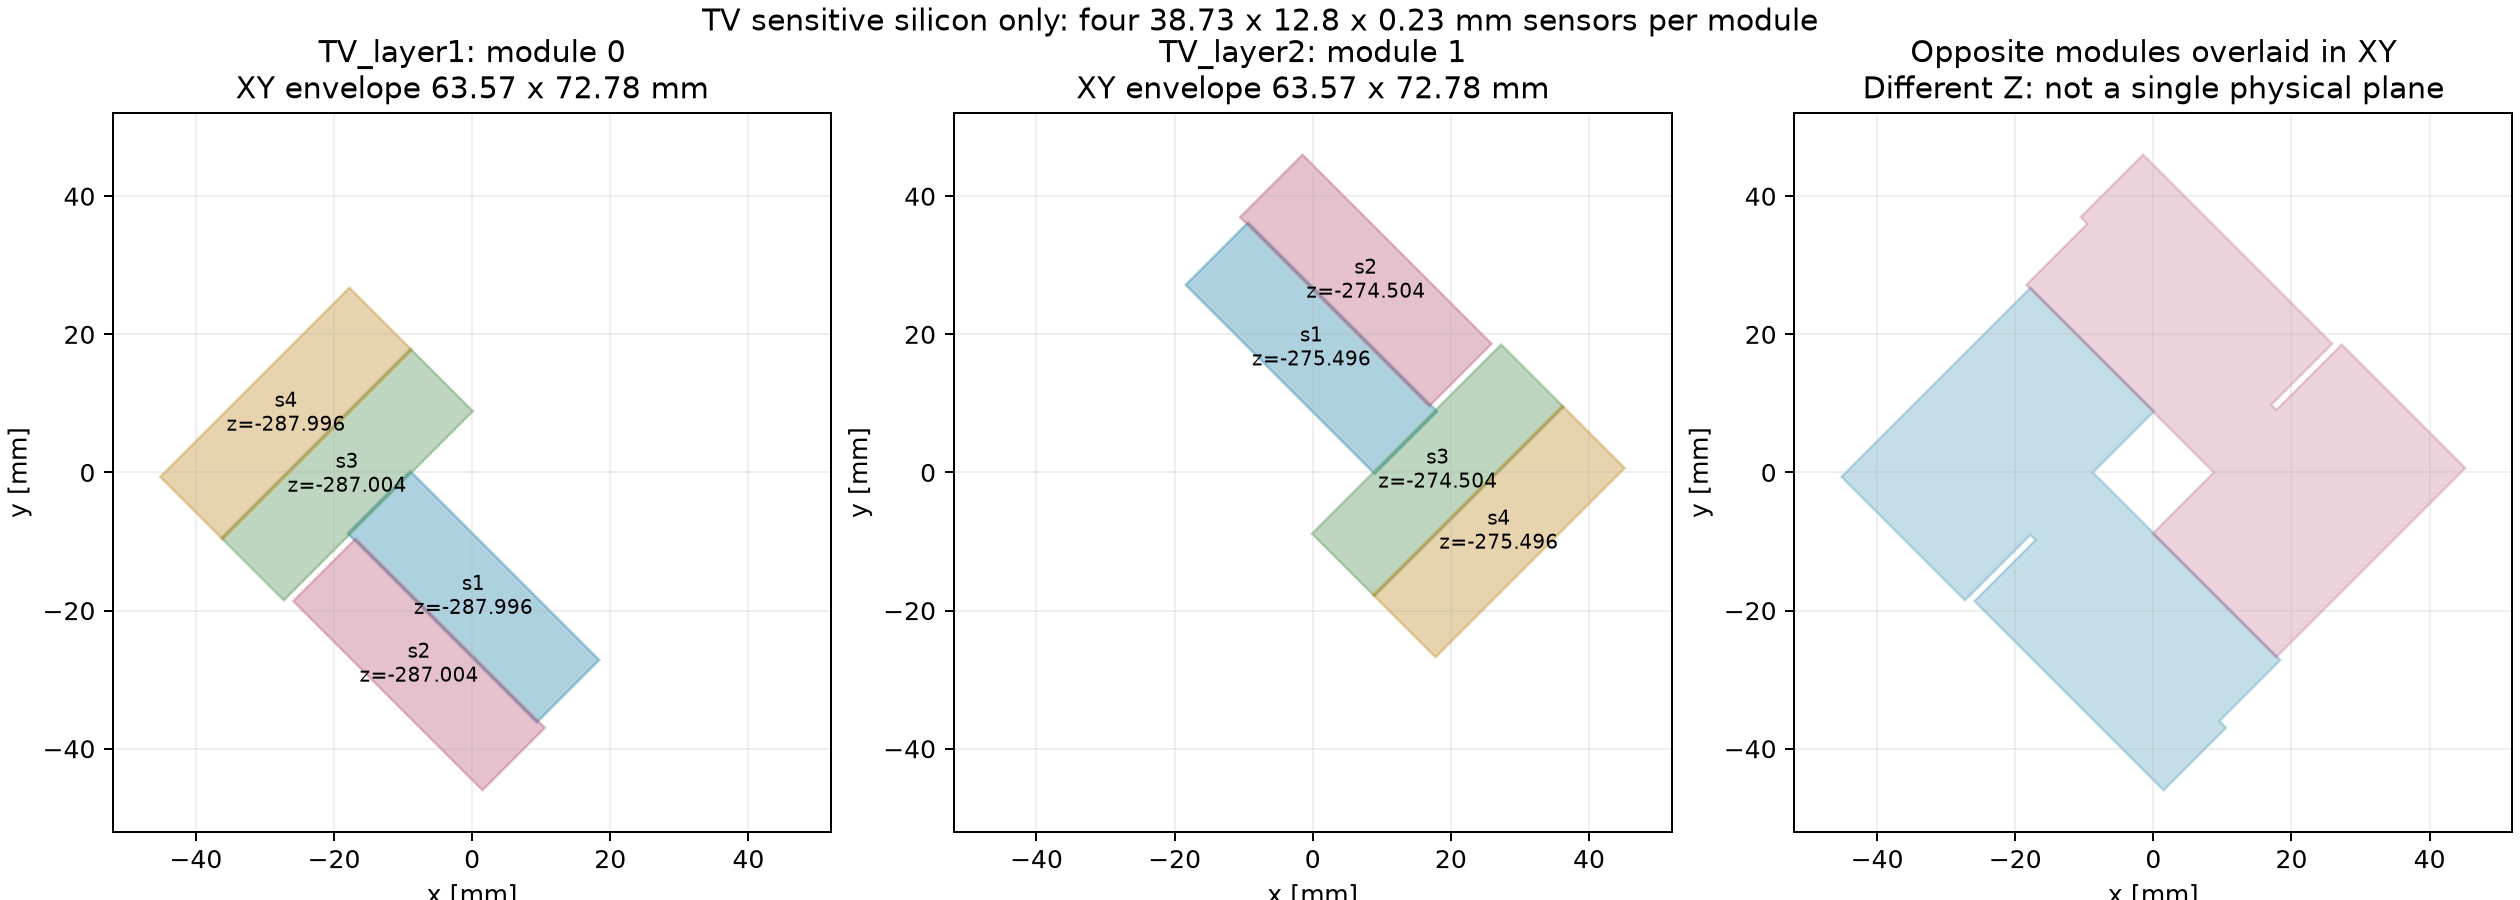
\includegraphics[width=\textwidth,height=.63\textheight,keepaspectratio]{../TV/review/tv_sensor_xy.png}\par
\small Select \texttt{TV:SensorSilicon} / \texttt{lvDet} in the source ROOT
hierarchy: 200 sensors, 38.73 $\times$ 12.8 $\times$ 0.23 mm each.\\[2mm]
Four sensors form one module, at two centre-$z$ positions 0.992 mm apart.
Only coplanar pairs are unioned; actual sensor gaps remain inactive.
\end{frame}

\begin{frame}{TV positioning: 100 sensor planes, 50 modules}
\centering
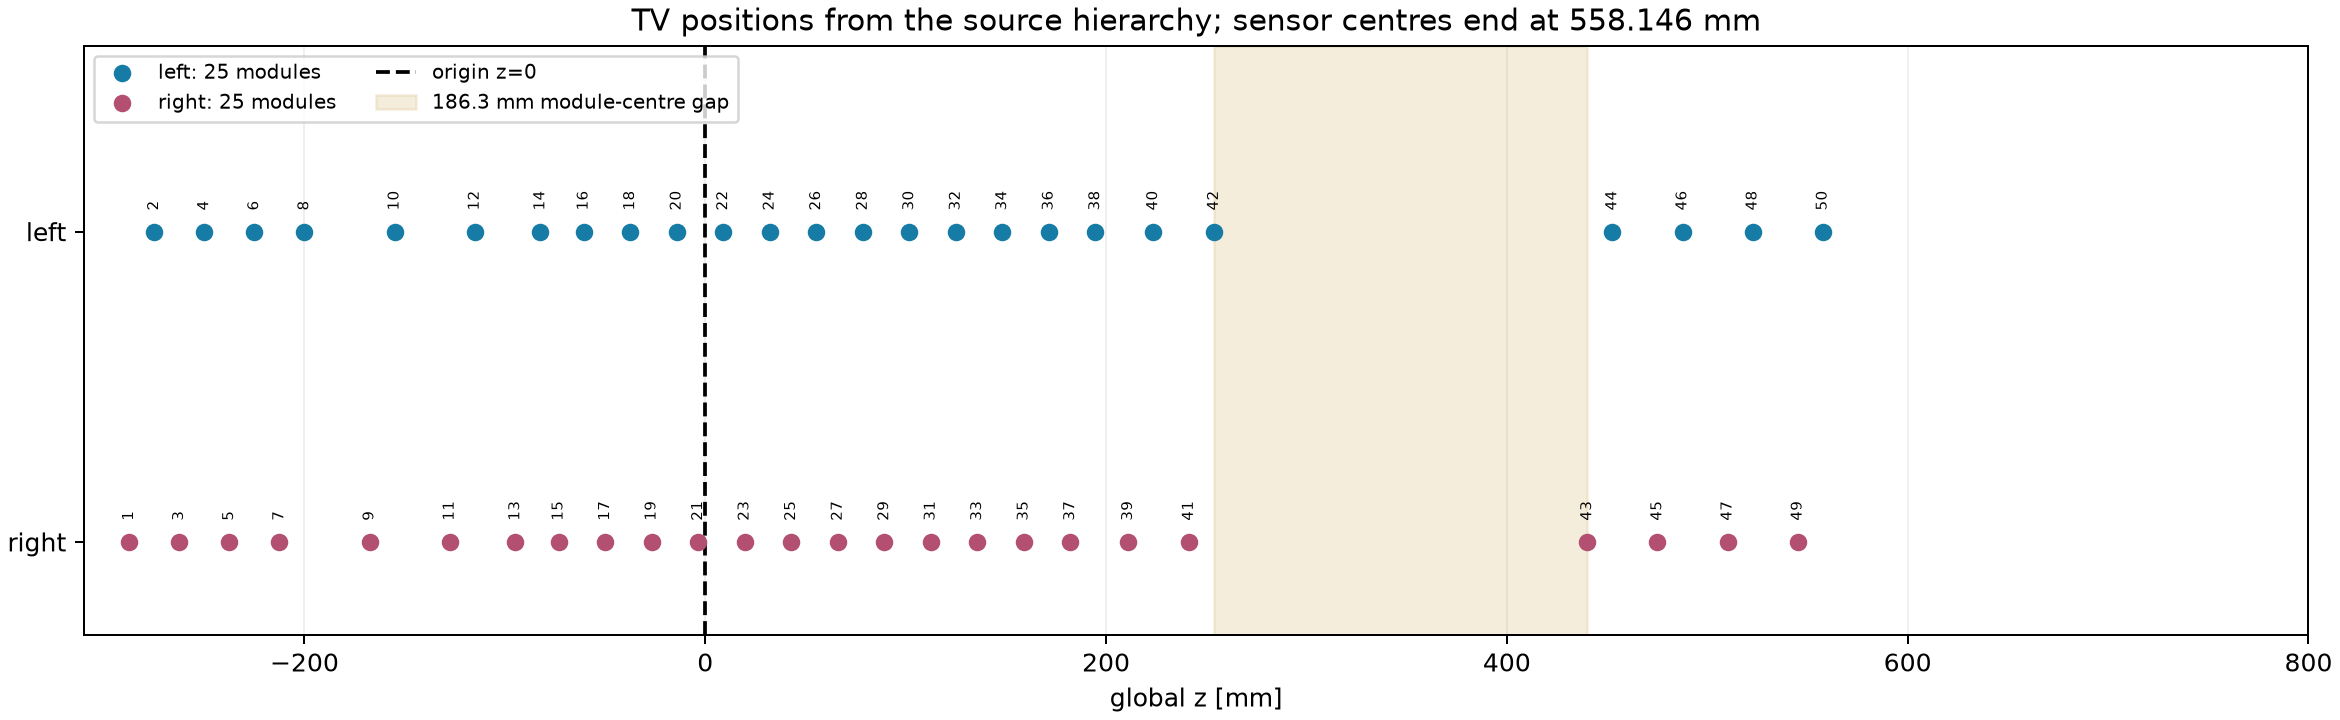
\includegraphics[width=\textwidth,height=.64\textheight,keepaspectratio]{../TV/review/tv_sensor_z.png}\par
\small Sensor centres span $-287.996$ to 558.146 mm. There is no sensitive
silicon around 700 or 780 mm in this input geometry.\\[2mm]
From the origin: 21 upstream modules cannot fire; 29 are reachable.
The 186.3 mm downstream gap is present in the ROOT hierarchy.
\end{frame}

\begin{frame}{TV emulation: mean hits and expected timing}
\centering
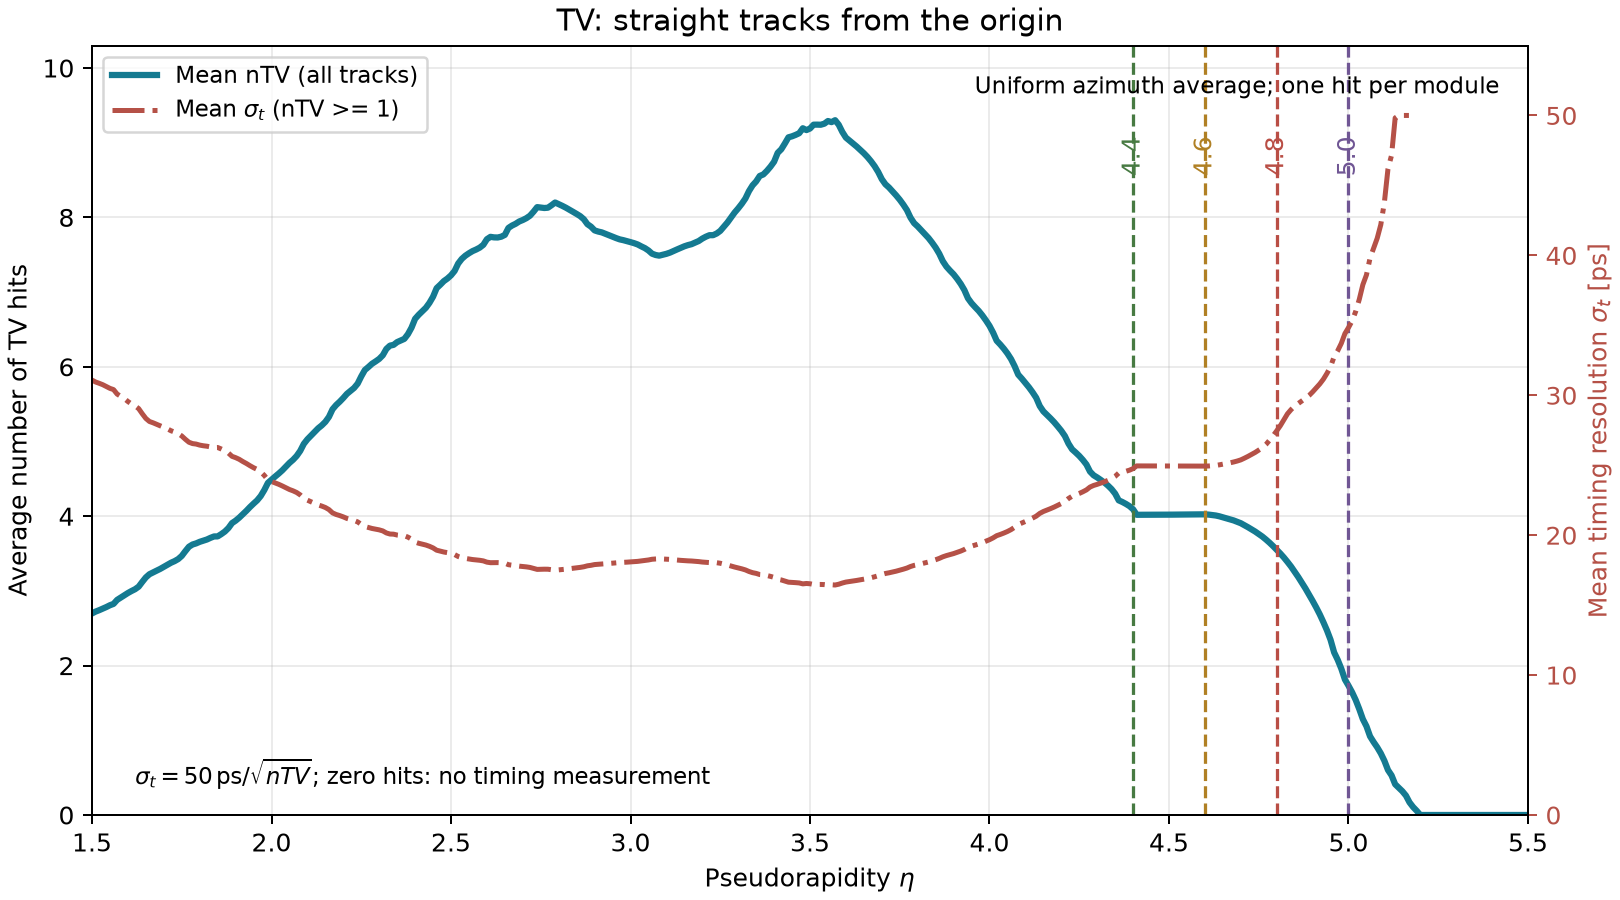
\includegraphics[width=.88\textwidth,height=.71\textheight,keepaspectratio]{../TV/geometry_review/tv_mean_hits_and_timing_vs_eta.png}\par
\small Straight origin rays, uniform azimuth. Timing uses
$\sigma_t=50\,\mathrm{ps}/\sqrt{n_{\rm TV}}$ per track, averaged for $n_{\rm TV}\geq1$.
Zero-hit tracks have no timing measurement.
\end{frame}

\begin{frame}{TV geometric efficiency for three and four hits}
\begin{columns}[T,onlytextwidth]
\column{.73\textwidth}
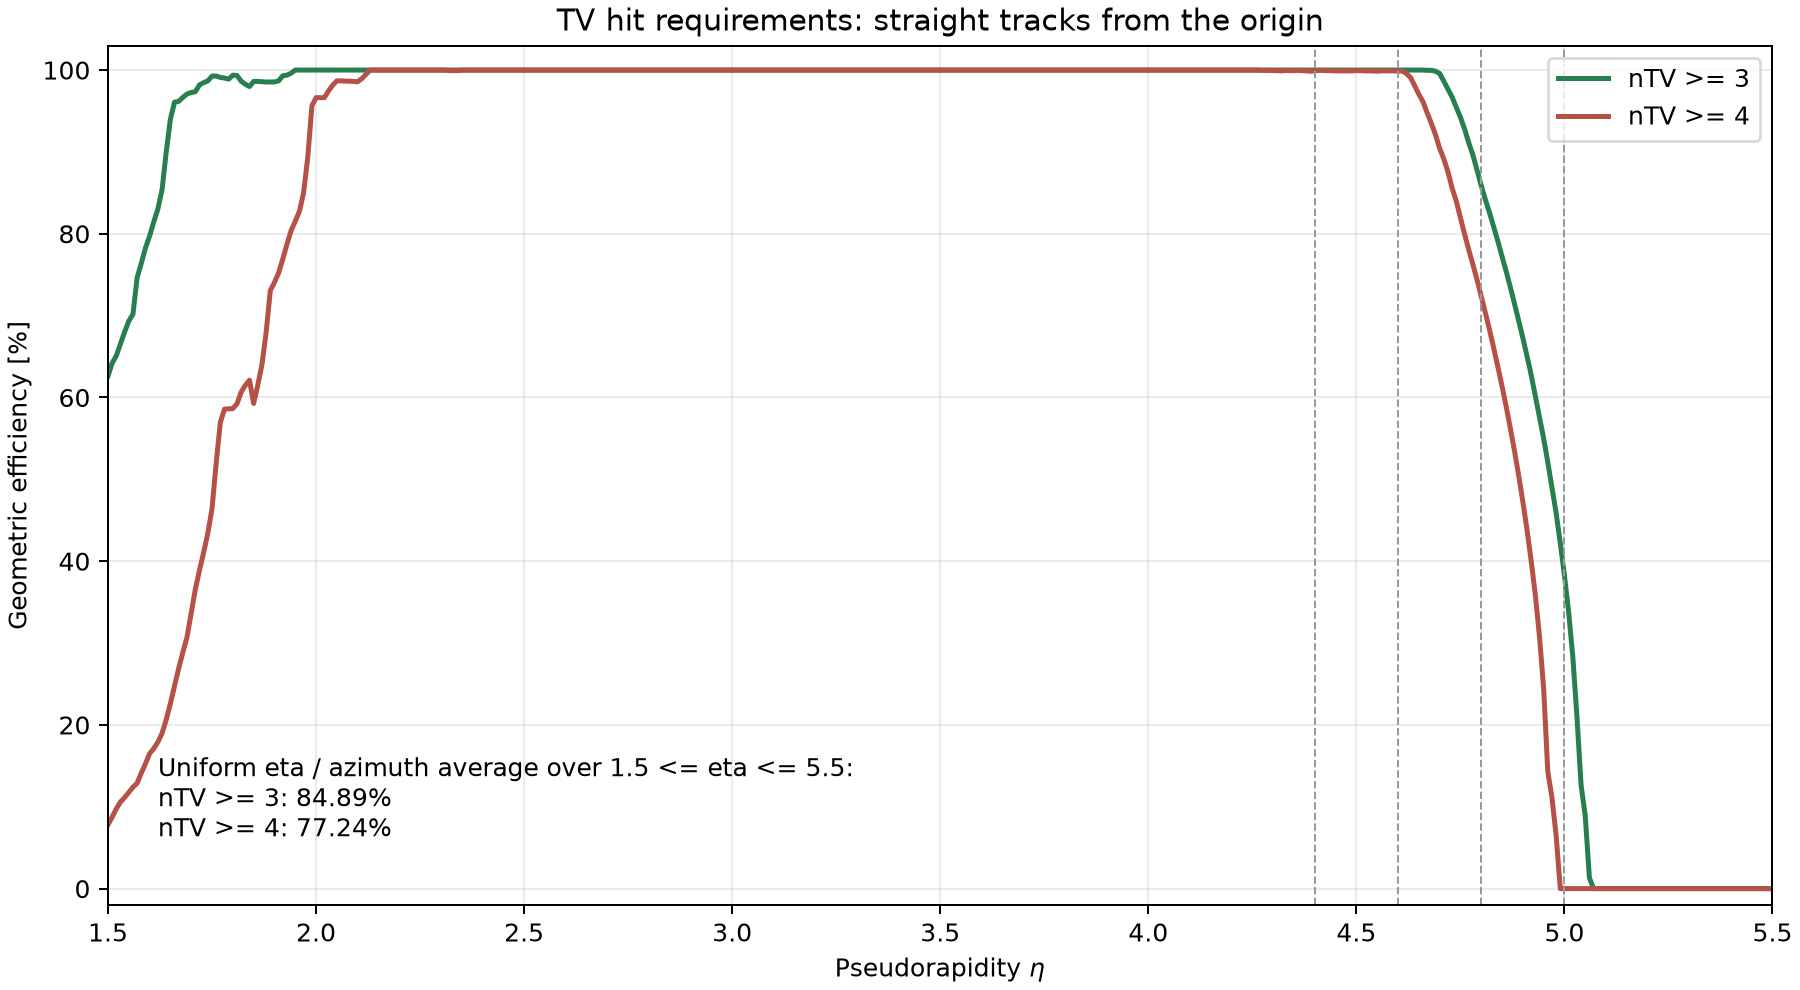
\includegraphics[width=\textwidth,height=.72\textheight,keepaspectratio]{../TV/geometry_review/tv_hit_cut_efficiency.png}
\column{.25\textwidth}
\small $1.5\leq\eta\leq5.5$\\[3mm]
Uniform $\eta$ and azimuth averages:\\[3mm]
$n_{\rm TV}\geq3$: \textbf{84.89\%}\\[3mm]
$n_{\rm TV}\geq4$: \textbf{77.24\%}\\[3mm]
1,154,880 rays.\\[3mm]
Numerical azimuth refinement changes efficiencies by less than 0.16 percentage points.
\end{columns}
\small No field, vertex spread, sensor inefficiency or reconstruction in this TV toy.
Physics-sample efficiencies need the actual track distribution.
\end{frame}

\begin{frame}{Field and transport validation}
\begin{itemize}
\item States are $(x,y,t_x,t_y,q/p)$ at a given $z$; positions in mm,
momentum in MeV/$c$, field in tesla.
\item Read Bx/By/Bz TH3 histograms; integrate with vectorized RK4.
No material scattering, energy loss or detector response.
\item Bundled reference map: $\int_0^{10000\,\rm mm} B_y\,dz = \FieldIntegral{}$ T m.
It is designated MagDown; MagUp reverses \emph{all three} components.
\item One transport per polarity is reused across six geometries: two transports,
not twelve. Counts and cuts keep geometry and polarity suffixes.
\item Tests cover straight rays, charge/field reversal, upstream exclusions,
counting groups, FT/UP border changes, MT cut boundaries and failed transport.
\item \textbf{118 tests passed} with the local ROOT field map, including the
two-polarity equivalence and track-order checks.
\end{itemize}
\small Sign-reversed maps are an idealization, not two independently measured maps.
\end{frame}

\begin{frame}[fragile]{One call labels every geometry and both polarities}
\begin{verbatim}
from xyshapes_detectors import PolarityComparison, MTSelection

service = PolarityComparison.from_files(
    "MagField/magnetic_field_v5r0.root",
    map_polarity="magdown",
    mt_selection=MTSelection(3, 10, 1, 6),
)
flags = service.label_tracks(states)
\end{verbatim}
\small Example output columns:\\[2mm]
\texttt{nFT\_up\_y8x6\_ft\_8\_8\_10\_withHole\_magup}\\
\texttt{nMP\_up\_y8x6\_ft\_8\_8\_10\_withHole\_magup}\\
\texttt{hasMT\_up\_y8x6\_ft\_8\_8\_10\_withHole\_magup}\\[3mm]
Equivalent MagDown columns are retained. The flags do not determine which
polarity was used in the data; choose that using the ntuple's metadata.
\end{frame}

\begin{frame}{Using the masks in decay studies}
\begin{itemize}
\item The field map, reusable masks, loader, transport, cuts and tests are in
the repository. No GDML extraction or ROOT installation is needed to consume them.
\item Reuse one service across bounded chunks. Prefix flags by daughter name;
preserve candidate rows and jagged track offsets when writing new branches.
\item Compare joint $(n_{\rm FT},n_{\rm MP})$ distributions and \texttt{hasMT}
between 8/8/10 and 10/10/12, holding UP and polarity fixed.
\item Compare $n_{\rm UP}$ for GDML, Y8 and Y8X6, holding FT and polarity fixed.
Combine with the chosen TV cut only at analysis level.
\item Next physics step: run on the selected decay ntuples, retain their
weights and denominator, and evaluate daughter and decay-level efficiencies.
\end{itemize}
\small Reproduction: \texttt{examples/create\_acceptance\_study\_slides.py}.\\
Usage: \texttt{docs/decay\_study\_quickstart.md}; API: \texttt{docs/geometry\_comparison.md}.
\end{frame}
\end{document}
